%% For camera-ready version:
% \documentclass[sigconf,natbib=false]{acmart}
%% For review version:
\documentclass[sigplan,natbib=false,review]{acmart}
\renewcommand\footnotetextcopyrightpermission[1]{}
\settopmatter{printfolios=true,printacmref=false}

%%
%% \BibTeX command to typeset BibTeX logo in the docs
\AtBeginDocument{%
  \providecommand\BibTeX{{%
    Bib\TeX}}}

%% Rights management information.  This information is sent to you
%% when you complete the rights form.  These commands have SAMPLE
%% values in them; it is your responsibility as an author to replace
%% the commands and values with those provided to you when you
%% complete the rights form.
\setcopyright{acmcopyright}
\copyrightyear{2024}
\acmYear{2024}
\acmDOI{XXXXXXX.XXXXXXX}

%%
%% Submission ID.
%% Use this when submitting an article to a sponsored event. You'll
%% receive a unique submission ID from the organizers
%% of the event, and this ID should be used as the parameter to this command.
%%\acmSubmissionID{123-A56-BU3}

%%
%% For managing citations, it is recommended to use bibliography
%% files in BibTeX format.
%%
%% You can then either use BibTeX with the ACM-Reference-Format style,
%% or BibLaTeX with the acmnumeric or acmauthoryear sytles, that include
%% support for advanced citation of software artefact from the
%% biblatex-software package, also separately available on CTAN.
%%
%% Look at the sample-*-biblatex.tex files for templates showcasing
%% the biblatex styles.
%%


%%
%% The majority of ACM publications use numbered citations and
%% references, obtained by selecting the acmnumeric BibLaTeX style.
%% The acmauthoryear BibLaTeX style switches to the "author year" style.
%%
%% If you are preparing content for an event
%% sponsored by ACM SIGGRAPH, you must use the acmauthoryear style of
%% citations and references.
%%
%% Bibliography style
\RequirePackage[
  datamodel=acmdatamodel,
  style=acmnumeric,
  ]{biblatex}

%% Declare bibliography sources (one \addbibresource command per source)
\addbibresource{references.bib}

%% My extra packages:
\usepackage{pgfplots} 
\usepackage{pgfplotstable}
\usepackage{filecontents}
\usepgfplotslibrary{colorbrewer}
\pgfplotsset{compat=1.16, cycle list/Set1-8} 
\usepackage{tikz}
\usetikzlibrary{
  automata,
  positioning,
  arrows, arrows.meta,
  calc, backgrounds, quotes,
  pgfplots.statistics, pgfplots.colorbrewer,
}
\tikzset{
  op/.style={
    font=\footnotesize,
    state,
    minimum size=40pt,
    fill=white,
  },
  head/.style={
    op,
    accepting,
  },
  edge/.style={
    ->,
    >={Stealth[round]},
  },
  pred/.style={
    edge,
  },
  anchorref/.style={
    edge,
    blue,
    dashed,
  },
  stepmarker/.style={
    font=\footnotesize,
    fill=black!10,
  },
  stepline/.style={
    edge,
    black!70,
    dotted,
    semithick,
    -,
  },
}

\usepackage{amsmath}
\usepackage{algorithm}
\usepackage{algpseudocodex}
\newcommand{\algorithmautorefname}{Algorithm}
\algrenewcommand\algorithmicforall{\textbf{for each}}
\usepackage[noabbrev,nameinlink,capitalize]{cleveref}
\newcounter{figcase}
\renewcommand{\thefigcase}{(\alph{figcase})}
\crefname{figcase}{case}{cases}
\Crefname{figcase}{Case}{Cases}
\creflabelformat{figcase}{#2#1#3}

\usepackage{booktabs}

\usepackage[acronym]{glossaries}
\makeglossaries{}
\newacronym{crdt}{CRDT}{Conflict-Free Replicated Data Type}
\newacronym{mvr}{MVR}{Multi-Valued Replicated Register}
\newacronym{lwwr}{LWWR}{Last-Write-Wins Register}
\newacronym{opid}{OpId}{Operation Id}
\newacronym{lifo}{LIFO}{last-in-first-out}
\newacronym{ot}{OT}{Operational Transformation}

\newcommand*{\fullref}[1]{\hyperref[{#1}]{\autoref*{#1}}}
\newcommand{\op}[3][op]{$\mathit{#1}_{#2}^{#3}$} % with op kind
\newcommand{\opid}[2]{$\mathit{_{#1}^{#2}}$}
\newcommand{\setop}[4][set]{$\mathit{#1_{#2}^{#3}}{(#4)}$}
\newcommand{\delop}[3][del]{$\mathit{#1_{#2}^{#3}}{()}$}
\newcommand{\undop}[5][undo]{$\mathit{#1_{#2}^{#3}}{(_{#4}^{#5})}$}
\newcommand{\redop}[5][redo]{$\mathit{#1_{#2}^{#3}}{(_{#4}^{#5})}$}
\newcommand{\restop}[5][rest]{$\mathit{#1_{#2}^{#3}}{(_{#4}^{#5})}$}
\newcommand{\stack}[1]{$[$#1$]$}
\def\setabbr{s}
\def\restabbr{rs}
\newcommand{\setopkind}{\textit{SetOp}}
\newcommand{\restopkind}{\textit{RestoreOp}}
\newcommand{\terminalopkind}{\textit{TerminalOp}}
\newcommand{\opidtrace}{\textit{OpIdTrace}}

%%
%% end of the preamble, start of the body of the document source.
\begin{document}

%%
%% The "title" command has an optional parameter,
%% allowing the author to define a "short title" to be used in page headers.
\title{Undo and Redo Support for Replicated Registers}

%%
%% The "author" command and its associated commands are used to define
%% the authors and their affiliations.
%% Of note is the shared affiliation of the first two authors, and the
%% "authornote" and "authornotemark" commands
%% used to denote shared contribution to the research.
\author{Leo Stewen}
% \authornote{Both authors contributed equally to this research.}
\email{lstwn@mailbox.org}
% \orcid{1234-5678-9012}
\affiliation{%
  \institution{Technical University of Munich}
  \country{Germany}
}

\author{Martin Kleppmann}
\email{martin@kleppmann.com}
\affiliation{%
 \institution{University of Cambridge}
 \country{United Kingdom}
}

%%
%% By default, the full list of authors will be used in the page
%% headers. Often, this list is too long, and will overlap
%% other information printed in the page headers. This command allows
%% the author to define a more concise list
%% of authors' names for this purpose.
% \renewcommand{\shortauthors}{Stewen et al.}

%%
%% The abstract is a short summary of the work to be presented in the
%% article.
\begin{abstract}
Undo and redo functionality is ubiquitous in collaboration software.
In single user settings, undo and redo are well understood.
However, when multiple users edit a document,
concurrency may arise, and the operation history can become non-linear.
This renders undo and redo more complex
both in terms of their semantics and implementation.

We survey the undo and redo semantics of current mainstream collaboration software
and derive principles for undo and redo behavior in a collaborative setting.
We then apply these principles to a simple \acrshort{crdt}, the \acrlong{mvr},
and present a novel undo and redo algorithm that implements the undo and redo
semantics that we believe are most consistent with users' expectations.
\end{abstract}

%%
%% The code below is generated by the tool at http://dl.acm.org/ccs.cfm.
%% Please copy and paste the code instead of the example below.
%%
\begin{CCSXML}
<ccs2012>
   <concept>
       <concept_id>10003120.10003130.10003233</concept_id>
       <concept_desc>Human-centered computing~Collaborative and social computing systems and tools</concept_desc>
       <concept_significance>500</concept_significance>
       </concept>
   <concept>
       <concept_id>10010147.10010919.10010172</concept_id>
       <concept_desc>Computing methodologies~Distributed algorithms</concept_desc>
       <concept_significance>300</concept_significance>
       </concept>
   <concept>
       <concept_id>10002951.10003152.10003166.10003172</concept_id>
       <concept_desc>Information systems~Remote replication</concept_desc>
       <concept_significance>300</concept_significance>
       </concept>
   <concept>
       <concept_id>10002951.10002952.10002971</concept_id>
       <concept_desc>Information systems~Data structures</concept_desc>
       <concept_significance>100</concept_significance>
       </concept>
 </ccs2012>
\end{CCSXML}

\ccsdesc[500]{Human-centered computing~Collaborative and social computing systems and tools}
\ccsdesc[300]{Computing methodologies~Distributed algorithms}
\ccsdesc[300]{Information systems~Remote replication}
\ccsdesc[100]{Information systems~Data structures}

%%
%% Keywords. The author(s) should pick words that accurately describe
%% the work being presented. Separate the keywords with commas.
\keywords{undo, redo, CRDT, eventual consistency, collaborative editing}

% \received{20 February 2007}
% \received[revised]{12 March 2009}
% \received[accepted]{5 June 2009}

%%
%% This command processes the author and affiliation and title
%% information and builds the first part of the formatted document.
\maketitle

\section{Introduction}\label{sec:introduction}

Collaborative editing is an essential feature in modern software.
\glspl*{crdt}~\cite{preguicca2018conflict} are gaining interest because they
enable collaboration in local-first software~\cite{kleppmann2019local},
that works with, but does not require the cloud to function.
They allow for concurrent editing of a shared document without requiring
central coordination while still guaranteeing strong eventual
consistency~\cite{shapiro2011comprehensive}.

As much as collaboration is a common feature today, so is undo and redo support.
Integrating it with \glspl*{crdt} is not trivial.
Although there are some published algorithms for undo and redo in \glspl*{crdt}
(see \cref{sec:related-work}),
their semantics do not match the behavior of current mainstream applications
as detailed in \cref{sec:semantics}.
We believe the semantics of mainstream applications are more in line with
user expectations for an undo feature, and therefore we propose an undo/redo
algorithm for \glspl{crdt} that follows this mainstream behavior.
It works on top of a \gls*{mvr}~\cite{shapiro2011comprehensive},
a core \gls*{crdt} that is often used as a basic
building block to build more complex \glspl*{crdt} via composition.
The intended environment for this algorithm is the Automerge~\cite{automerge} library,
which is a JSON \gls*{crdt} that is based on \glspl*{mvr}.

\section{Semantics of Undo/Redo with Multiple Users}\label{sec:semantics}

\begin{figure}
\centering
\begin{tikzpicture}[node distance=0.23cm]
  \coordinate (c1) at (0,0);

  \tikzset{
    canvas/.style={
      rectangle,
      draw,
      anchor = west,
      inner sep = 4pt,
    },
    rect/.style={
      rectangle,
      minimum width = 1.2cm, 
      minimum height = 0.5cm,
      inner sep = 0.1cm,
      text = white,
      fill = #1,
    },
    optrans/.style={
      <-,bend right=90,>={Stealth[round]},
      swap,
      black!70,
    },
    next/.style={
      <-,
      >={Stealth[round]},
    },
    caselabel/.style={
      rectangle,
      draw,
      fill=white,
      minimum width = 238.5pt,
      % just for left align of text
      text width=220pt,
    },
  }

  \def\black{black}
  \def\green{green!60!black}
  \def\red{red}
  \def\upperoffset{28pt}
  \def\casemargin{28pt}
  \def\caselabeldist{5pt}

  % two registers, global undo

  \node[
    canvas,
    % label={[]above:(a1)},
  ] (a1) at (c1) {
    \begin{tikzpicture}[node distance=3pt]
      \node[
          rect=\black,
        ] (r1) at (0,0) {\vphantom{bg}black};
      \node[
          rect=\black,
          below = of r1,
        ] (r2) {\vphantom{bg}black};
    \end{tikzpicture}
  };

  \node[
    canvas,
    % label={[]above:(a2)},
    right = of a1,
  ] (a2) {
    \begin{tikzpicture}[node distance=3pt]
      \node[
          rect=\red,
        ] (r1) at (0,0) {\vphantom{bg}red};
      \node[
          rect=\black,
          below = of r1,
        ] (r2) {\vphantom{bg}black};
    \end{tikzpicture}
  } edge [next] (a1);

  \node[
    canvas,
    % label={[]above:(a3)},
    right = of a2,
  ] (a3) {
    \begin{tikzpicture}[node distance=3pt]
      \node[
          rect=\red,
        ] (r1) at (0,0) {\vphantom{bg}red};
      \node[
          rect=\green,
          below = of r1,
        ] (r2) {\vphantom{bg}green};
    \end{tikzpicture}
  } edge [next] (a2);

  \node[
    canvas,
    % label={[]above:(a4)},
    right = of a3,
  ] (a4) {
    \begin{tikzpicture}[node distance=3pt]
      \node[
          rect=\red,
        ] (r1) at (0,0) {\vphantom{bg}red};
      \node[
          rect=\black,
          below = of r1,
        ] (r2) {\vphantom{bg}black};
    \end{tikzpicture}
  } edge [next] (a3);

  \node[
    canvas,
    % label={[]above:(a5)},
    right = of a4,
  ] (a5) {
    \begin{tikzpicture}[node distance=3pt]
      \node[
          rect=\red,
        ] (r1) at (0,0) {\vphantom{bg}red};
      \node[
          rect=\green,
          below = of r1,
        ] (r2) {\vphantom{bg}green};
    \end{tikzpicture}
  } edge [next] (a4);

  % two registers, local undo

  \node[
    canvas,
    % label={[]above:(b1)},
    below=\casemargin of a1,
  ] (b1) {
    \begin{tikzpicture}[node distance=3pt]
      \node[
          rect=\black,
        ] (r1) at (0,0) {\vphantom{bg}black};
      \node[
          rect=\black,
          below = of r1,
        ] (r2) {\vphantom{bg}black};
    \end{tikzpicture}
  };

  \node[
    canvas,
    % label={[]above:(b2)},
    right = of b1,
  ] (b2) {
    \begin{tikzpicture}[node distance=3pt]
      \node[
          rect=\red,
        ] (r1) at (0,0) {\vphantom{bg}red};
      \node[
          rect=\black,
          below = of r1,
        ] (r2) {\vphantom{bg}black};
    \end{tikzpicture}
  } edge [next] (b1);

  \node[
    canvas,
    % label={[]above:(b3)},
    right = of b2,
  ] (b3) {
    \begin{tikzpicture}[node distance=3pt]
      \node[
          rect=\red,
        ] (r1) at (0,0) {\vphantom{bg}red};
      \node[
          rect=\green,
          below = of r1,
        ] (r2) {\vphantom{bg}green};
    \end{tikzpicture}
  } edge [next] (b2);

  \node[
    canvas,
    % label={[]above:(b4)},
    right = of b3,
  ] (b4) {
    \begin{tikzpicture}[node distance=3pt]
      \node[
          rect=\black,
        ] (r1) at (0,0) {\vphantom{bg}black};
      \node[
          rect=\green,
          below = of r1,
        ] (r2) {\vphantom{bg}green};
    \end{tikzpicture}
  } edge [next] (b3);

  \node[
    canvas,
    % label={[]above:(b5)},
    right = of b4,
  ] (b5) {
    \begin{tikzpicture}[node distance=3pt]
      \node[
          rect=\red,
        ] (r1) at (0,0) {\vphantom{bg}red};
      \node[
          rect=\green,
          below = of r1,
        ] (r2) {\vphantom{bg}green};
    \end{tikzpicture}
  } edge [next] (b4);

  % one register, global undo

  \node[
    canvas,
    % label={[]above:(3a)},
    below=\casemargin of b1,
  ] (3a) {
    \begin{tikzpicture}[node distance=3pt]
      \node[
          rect=\black,
        ] (r1) at (0,0) {\vphantom{bg}black};
    \end{tikzpicture}
  };

  \node[
    canvas,
    % label={[]above:(c2)},
    right = of 3a,
  ] (c2) {
    \begin{tikzpicture}[node distance=3pt]
      \node[
          rect=\red,
        ] (r1) at (0,0) {\vphantom{bg}red};
    \end{tikzpicture}
  } edge [next] (3a);

  \node[
    canvas,
    % label={[]above:(c3)},
    right = of c2,
  ] (c3) {
    \begin{tikzpicture}[node distance=3pt]
      \node[
          rect=\green,
        ] (r1) at (0,0) {\vphantom{bg}green};
    \end{tikzpicture}
  } edge [next] (c2);

  \node[
    canvas,
    % label={[]above:(c4)},
    right = of c3,
  ] (c4) {
    \begin{tikzpicture}[node distance=3pt]
      \node[
          rect=\red,
        ] (r1) at (0,0) {\vphantom{bg}red};
    \end{tikzpicture}
  } edge [next] (c3);

  \node[
    canvas,
    % label={[]above:(c5)},
    right = of c4,
  ] (c5) {
    \begin{tikzpicture}[node distance=3pt]
      \node[
          rect=\green,
        ] (r1) at (0,0) {\vphantom{bg}green};
    \end{tikzpicture}
  } edge [next] (c4);

  % one register, local undo

  \node[
    canvas,
    % label={[]above:(d1)},
    below=\casemargin of 3a,
  ] (d1) {
    \begin{tikzpicture}[node distance=3pt]
      \node[
          rect=\black,
        ] (r1) at (0,0) {\vphantom{bg}black};
    \end{tikzpicture}
  };

  \node[
    canvas,
    % label={[]above:(d2)},
    right = of d1,
  ] (d2) {
    \begin{tikzpicture}[node distance=3pt]
      \node[
          rect=\red,
        ] (r1) at (0,0) {\vphantom{bg}red};
    \end{tikzpicture}
  } edge [next] (d1);

  \node[
    canvas,
    % label={[]above:(d3)},
    right = of d2,
  ] (d3) {
    \begin{tikzpicture}[node distance=3pt]
      \node[
          rect=\green,
        ] (r1) at (0,0) {\vphantom{bg}green};
    \end{tikzpicture}
  } edge [next] (d2);

  \node[
    canvas,
    % label={[]above:(4d)},
    right = of d3,
  ] (4d) {
    \begin{tikzpicture}[node distance=3pt]
      \node[
          rect=\black,
        ] (r1) at (0,0) {\vphantom{bg}black};
    \end{tikzpicture}
  } edge [next] (d3);

  \node[
    canvas,
    % label={[]above:(d4)},
    right = of 4d,
  ] (d4) {
    \begin{tikzpicture}[node distance=3pt]
      \node[
          rect=\green,
        ] (r1) at (0,0) {\vphantom{bg}green};
    \end{tikzpicture}
  } edge [next] (4d);

  % one register, remote op blocks undo

  \node[
    canvas,
    % label={[]above:(e1)},
    below=\casemargin of d1,
  ] (e1) {
    \begin{tikzpicture}[node distance=3pt]
      \node[
          rect=\black,
        ] (r1) at (0,0) {\vphantom{bg}black};
    \end{tikzpicture}
  };

  \node[
    canvas,
    % label={[]above:(e2)},
    right = of e1,
  ] (e2) {
    \begin{tikzpicture}[node distance=3pt]
      \node[
          rect=\red,
        ] (r1) at (0,0) {\vphantom{bg}red};
    \end{tikzpicture}
  } edge [next] (e1);

  \node[
    canvas,
    % label={[]above:(e3)},
    right = of e2,
  ] (e3) {
    \begin{tikzpicture}[node distance=3pt]
      \node[
          rect=\green,
        ] (r1) at (0,0) {\vphantom{bg}green};
    \end{tikzpicture}
  } edge [next] (e2);

  \node[
    canvas,
    % label={[]above:(e4)},
    right = of e3,
  ] (e4) {
    \begin{tikzpicture}[node distance=3pt]
      \node[
          rect=\green,
        ] (r1) at (0,0) {\vphantom{bg}green};
    \end{tikzpicture}
  } edge [next] (e3);

  \node[
    canvas,
    % label={[]above:(e5)},
    right = of e4,
  ] (e5) {
    \begin{tikzpicture}[node distance=3pt]
      \node[
          rect=\green,
        ] (r1) at (0,0) {\vphantom{bg}green};
    \end{tikzpicture}
  } edge [next] (e4);

  % divider lines and ops

  \coordinate (d1s) at ($(a1.north)!0.5!(a2.north)+(0,+\upperoffset)$);
  \coordinate (da5) at ($(e1.south)!0.5!(e2.south)+(0,0)$);

  \coordinate (d2s) at ($(a2.north)!0.5!(a3.north)+(0,+\upperoffset)$);
  \coordinate (db5) at ($(e2.south)!0.5!(e3.south)+(0,0)$);

  \coordinate (d3s) at ($(a3.north)!0.5!(a4.north)+(0,+\upperoffset)$);
  \coordinate (dc5) at ($(e3.south)!0.5!(e4.south)+(0,0)$);

  \coordinate (d4s) at ($(a4.north)!0.5!(a5.north)+(0,+\upperoffset)$);
  \coordinate (dd4) at ($(e4.south)!0.5!(e5.south)+(0,0)$);

  \draw[stepline] (d1s) -- (da5);
  \draw[stepline] (d2s) -- (db5);
  \draw[stepline] (d3s) -- (dc5);
  \draw[stepline] (d4s) -- (dd4);

  \draw (a2.north)+(-0.2cm,+\upperoffset) edge ["A set",optrans] ($(a1.north)+(0,+\upperoffset)$);
  \draw (a3.north)+(-0.2cm,+\upperoffset) edge ["B set",optrans] ($(a2.north)+(0,+\upperoffset)$);
  \draw (a4.north)+(-0.2cm,+\upperoffset) edge ["A undo",optrans] ($(a3.north)+(0,+\upperoffset)$);
  \draw (a5.north)+(-0.2cm,+\upperoffset) edge ["A redo",optrans] ($(a4.north)+(0,+\upperoffset)$);

  % case labels

  \node[caselabel,above=\caselabeldist of a3] {
    \refstepcounter{figcase}\label{fig:two-reg-global}\thefigcase{} Two registers, global undo
  };

  \node[caselabel,above=\caselabeldist of b3] {
    \refstepcounter{figcase}\label{fig:two-reg-local}\thefigcase{} Two registers, local undo
  };

  \node[caselabel,above=\caselabeldist of c3] {
    \refstepcounter{figcase}\label{fig:one-reg-global}\thefigcase{} One register, global undo
  };

  \node[caselabel,above=\caselabeldist of d3] {
    \refstepcounter{figcase}\label{fig:one-reg-local}\thefigcase{} One register, local undo
  };

  \node[caselabel,above=\caselabeldist of e3] {
    \refstepcounter{figcase}\label{fig:one-reg-block}\thefigcase{} One register, remote operation blocks undo
  };
  
\end{tikzpicture}
\caption{
  Different semantics of undo and redo with two users A and B collaboratively
  editing one (two) register(s).
}\label{fig:intro-example}
\end{figure}

To illustrate the possible semantics of undo and redo with multiple users,
we consider replicated registers that are used to store the fill color
of a rectangle, for instance, on a slide of a presentation deck.
\cref{fig:intro-example} illustrates possible behaviors of undo and redo.
\Cref{fig:two-reg-global,fig:two-reg-local} deal with an application 
with two registers (rectangles) and
\Cref{fig:one-reg-global,fig:one-reg-local,fig:one-reg-block} show an
application with one register. 
We assume that all operations are instantly synced to the other peer and the
operations run sequentially, disregarding concurrency for now.
We distinguish between the following undo behaviors:

\textbf{Global undo.}
In \cref{fig:intro-example}~\ref{fig:two-reg-global},
user $A$ changes the upper rectangle's color
to red, then user $B$ sets the lower rectangle's color to green.
When $A$ subsequently performs an undo, it undoes the most recent operation
\emph{by any user}, i.e., it undoes $B$'s operation by setting the lower
rectangle back to black.
$A$'s redo operation restores the lower rectangle to green.

\Cref{fig:one-reg-global} shows the analogous scenario in which user $A$
and $B$ update the same rectangle.
When $A$ performs an undo, it undoes the most recent operation
again \emph{by any user}, changing the rectangle from green back to red.

\textbf{Local undo.}
In \cref{fig:intro-example}~\ref{fig:two-reg-global},
user $A$ changes the upper rectangle to red,
then user $B$ sets the lower rectangle to green.
Afterwards, user $A$ performs an undo, which undoes the most recent operation
\emph{by $A$ itself}, i.e., changing the upper rectangle back to black.
$A$'s subsequent redo restores the upper rectangle back to red.

In \Cref{fig:one-reg-local}, there is only one rectangle.
First, user $A$ changes it to red, then user $B$ changes it to green.
Subsequently, $A$ performs an undo, and like in the two-register case, this
restores the value of the register to the state before the most recent operation
\emph{by $A$ itself}, i.e., changing it back to black.
When then $A$ performs its redo, the state prior to the undo is restored, i.e.,
green.

\textbf{Remote operation blocks undo.}
In \cref{fig:intro-example}~\ref{fig:one-reg-block}, if user $A$ tries to
perform an undo in a state where the most recent operation is by a different user,
the undo function is disabled for $A$.

To sum it up, \emph{local undo} undoes the last operation
performed by the same user who issues the undo.
On the other hand, \emph{global undo} undoes the last operation
performed by any user.
In any case, however, a redo restores to the state prior to its corresponding undo,
regardless of the origin of the operations that constitute this state.

%% no concurrency for now
% The rectangle's color is stored in a \gls*{lwwr}~\cite{shapiro2011comprehensive}.
% If multiple users concurrently set its color, the register picks one of
% the concurrently assigned colors arbitrarily as the merged final state.
% The difference between the upper scenario (1a-1e) and the lower scenario (2a-2e)
% is that in the former, $A$ and $B$ do not work on the same register:
% $A$ works exclusively on the upper rectangle and $B$ on the lower one.
% In the lower scenario, $A$ and $B$ collaborate on the same rectangle.
% All operations are immediately synced to the other user before another change
% is introduced, avoiding concurrency for now.
% Hence, both users have seen the same progression of colors.

%% software survey

We tested the behavior of undo and redo in Google Sheets, Google Slides,
Microsoft Excel Online, Microsoft PowerPoint Online, Figma and Miro Boards.
In spreadsheets (Google Sheets and Microsoft Excel Online)
we test a register by setting the value of a single cell instead of recoloring
a rectangle.
All applications we tested exhibit local undo behavior as shown in
\cref{fig:intro-example}~\ref{fig:two-reg-local}~and~\ref{fig:one-reg-local},
except for Miro Boards, which blocks undo every time an operation
by another user is received, as illustrated
in \cref{fig:intro-example}~\ref{fig:one-reg-block}.
The most common implementations of multi-user undo for a register
can be characterized by the following principles:

\begin{itemize}
  \item \textbf{Local undo}:
    An undo by a user undoes her own last operation on a register,
    thereby possibly also undoing operations by other users on that register,
    if they lie temporally in between her last operation and the time of
    issuing the undo.
  \item \textbf{Undo Redo Neutrality}~\cite{figma2019multiplayer}:
    Assume a register is in state $s$.
    A sequence of $n$ undo operations followed by a sequence of $n$ redo operations
    should restore state $s$.
\end{itemize}

The last principle captures a common usage pattern of undo and redo.
Often users want to look at a past version of a document and then restore
to the most recent version without changing anything.

%% argue for local instead of global undo behavior

We think that most applications settled for local undo behavior because
global undo implicitly assumes users being aware of remote changes, too,
all while editing a document, and this is a fairly strong assumption to make.
\Cref{fig:intro-example}~\ref{fig:two-reg-global} demonstrates this issue
if we think about the two registers living in different parts of a document,
e.g., the upper rectangle is on a slide user $A$ is currently looking at
and the lower rectangle is on a different slide user $B$ is editing.
With global undo, $A$ may be surprised to see no immediate effect of her undo
because it reverted $B$'s green coloring on a different slide,
while actually expecting her last change to be undone for fixing
an accidental change of hers.
On the other hand, $B$ may surprised to learn that her last
change was undone for no obvious reason.
With more users editing collaboratively, the problem exacerbates, as the
share of remote operations tends to increase with the number of users.
Hence, we are convinced that the strongest reasonable assumption is to
assume that users are aware of their own changes.
Since we think that users favor predictable and consistent semantics,
undo behavior with one register should follow local undo behavior as well and
not depend on the number of registers involved.

Furthermore, global undo in a \gls{crdt} context suffers from additional problems.
It is possible that multiple users concurrently undo or redo overlapping subsets
of operations, leading to potentially confusing states.
Local undo does not suffer from this problem, since users can only undo 
their own operations.
Finally, global undo presumes that users agree on a total order of operations.
If the total order is determined by (logical) timestamps on operations,
this order is cannot be final.
Then, it is possible that a user undoes the operations
it knows in some timestamp interval $[t_1, t_2]$, and subsequently receives
a remote operation with a timestamp $t_{op}$ that falls within the
interval ($t_1 < t_{op} < t_2$).
It is unclear how an algorithm should handle this situation without leading
to further unexpected states.
The fact that most non-\gls{crdt} software chooses local undo over global undo
despite not being affected by this, makes another case for following their lead.

\section{Background on MVRs}\label{sec:background}

\begin{figure*}[!ht]
\centering
\begin{tikzpicture}
  \tikzset{
    font=\footnotesize,
    op/.style={
      state,
    },
  }

  \node [anchor=west] at (0.0,5.4) {Actor A:};
  \node [anchor=west] at (0.0,1.4) {Actor B:};

  \def\dist{1.4cm}

  \node [rectangle,draw,anchor=west] (a1) at (0,4) {
    \begin{tikzpicture}[node distance=\dist]
      \node[op] (opa1) {\setop{1}{A}{1}};
      \node[head, right of=opa1] (opb2) {\setop{2}{B}{2}} edge [pred] (opa1);

      \node[below=of opb2,yshift=+1.3cm] (vals) {$\text{MVR}: [2]$};
      \node[stepmarker,anchor=south west] at (0,-1.25) {(1)};
    \end{tikzpicture}
  };

  \node [rectangle,draw,anchor=west] (b1) at (0,0) {
    \begin{tikzpicture}[node distance=\dist]
      \node[op] (opa1) {\setop{1}{A}{1}};
      \node[head, right of=opa1] (opb2) {\setop{2}{B}{2}} edge [pred] (opa1);

      \node[below=of opb2,yshift=+1.3cm] (vals) {$\text{MVR}: [2]$};
      \node[stepmarker,anchor=south west] at (0,-1.25) {(1)};
    \end{tikzpicture}
  };

  \node [rectangle,draw,anchor=west] (a2) at (3.05,4) {
    \begin{tikzpicture}[node distance=\dist]
      \node[op] (opa1) {\setop{1}{A}{1}};
      \node[op, right of=opa1] (opb2) {\setop{2}{B}{2}} edge [pred] (opa1);
      \node[head, right of=opb2] (opa3) {\setop{3}{A}{3}} edge [pred] (opb2);

      \node[below=of opa3,yshift=+1.3cm] (vals) {$\text{MVR}: [3]$};
      \node[stepmarker,anchor=south west] at (0,-1.25) {(2a)};
    \end{tikzpicture}
  };

  \node [rectangle,draw,anchor=west] (b2) at (3.05,0) {
    \begin{tikzpicture}[node distance=\dist]
      \node[op] (opa1) {\setop{1}{A}{1}};
      \node[op, right of=opa1] (opb2) {\setop{2}{B}{2}} edge [pred] (opa1);
      \node[head, right of=opb2] (opb3) {\setop{3}{B}{4}} edge [pred] (opb2);

      \node[below=of opa3,yshift=+1.3cm] (vals) {$\text{MVR}: [4]$};
      \node[stepmarker,anchor=south west] at (0,-1.25) {(2b)};
    \end{tikzpicture}
  };

  \node [rectangle,draw,anchor=west] (a3) at (7.5,4) {
    \begin{tikzpicture}[node distance=\dist]
      \node[op] (opa1) {\setop{1}{A}{1}};
      \node[op, right of=opa1] (opb2) {\setop{2}{B}{2}} edge [pred] (opa1);
      \node[head, above right=of opb2, xshift=-0.4cm, yshift=-1.2cm] (opa3) {\setop{3}{A}{3}} edge [pred] (opb2);
      \node[head, below right=of opb2, xshift=-0.4cm, yshift=+1.2cm] (opb3) {\setop{3}{B}{4}} edge [pred] (opb2);

      \node[below=of opb3,yshift=+1.3cm,xshift=-0.17cm] (vals) {$\text{MVR}: [4,3]$};
      \node[stepmarker,anchor=south west] at (0,-1.76) {(3)};
    \end{tikzpicture}
  };

  \node [rectangle,draw,anchor=west] (b3) at (7.5,0) {
    \begin{tikzpicture}[node distance=\dist]
      \node[op] (opa1) {\setop{1}{A}{1}};
      \node[op, right of=opa1] (opb2) {\setop{2}{B}{2}} edge [pred] (opa1);
      \node[head, above right=of opb2, xshift=-0.4cm, yshift=-1.2cm] (opa3) {\setop{3}{A}{3}} edge [pred] (opb2);
      \node[head, below right=of opb2, xshift=-0.4cm, yshift=+1.2cm] (opb3) {\setop{3}{B}{4}} edge [pred] (opb2);

      \node[below=of opb3,yshift=+1.3cm,xshift=-0.17cm] (vals) {$\text{MVR}: [4,3]$};
      \node[stepmarker,anchor=south west] at (0,-1.76) {(3)};
    \end{tikzpicture}
  };

  \node [rectangle,draw,anchor=west] (a4) at (11.93,4) {
    \begin{tikzpicture}[node distance=\dist]
      \node[op] (opa1) {\setop{1}{A}{1}};
      \node[op, right of=opa1] (opb2) {\setop{2}{B}{2}} edge [pred] (opa1);
      \node[op, above right=of opb2, xshift=-0.4cm, yshift=-1.2cm] (opa3) {\setop{3}{A}{3}} edge [pred] (opb2);
      \node[op, below right=of opb2, xshift=-0.4cm, yshift=+1.2cm] (opb3) {\setop{3}{B}{4}} edge [pred] (opb2);
      \node[head, below right=of opa3, xshift=-0.4cm, yshift=+1.2cm] (opa4) {\delop{4}{A}} edge [pred] (opa3) edge [pred] (opb3);

      \node[below=of opa4,yshift=+1.3cm] (vals) {$\text{MVR}: []$};
      \node[stepmarker,anchor=south west] at (0,-1.34) {(4)};
    \end{tikzpicture}
  };

  \node [rectangle,draw,anchor=west] (b4) at (11.93,0) {
    \begin{tikzpicture}[node distance=\dist]
      \node[op] (opa1) {\setop{1}{A}{1}};
      \node[op, right of=opa1] (opb2) {\setop{2}{B}{2}} edge [pred] (opa1);
      \node[op, above right=of opb2, xshift=-0.4cm, yshift=-1.2cm] (opa3) {\setop{3}{A}{3}} edge [pred] (opb2);
      \node[op, below right=of opb2, xshift=-0.4cm, yshift=+1.2cm] (opb3) {\setop{3}{B}{4}} edge [pred] (opb2);
      \node[head, below right=of opa3, xshift=-0.4cm, yshift=+1.2cm] (opa4) {\delop{4}{A}} edge [pred] (opa3) edge [pred] (opb3);

      \node[below=of opa4,yshift=+1.3cm] (vals) {$\text{MVR}: []$};
      \node[stepmarker,anchor=south west] at (0,-1.34) {(4)};
    \end{tikzpicture}
  };

  \draw [|-|,draw=green!80!black!80,dashed] 
    ($(a1.south west)!0.5!(b1.north west)$) -- ($(a1.south east)!0.5!(b1.north east)$);
  \draw [|-|,draw=red] 
    ($(a1.south east)!0.5!(b1.north east)$) -- 
    node[above,color=red] {Network Partition}
    ($(a3.south west)!0.5!(b3.north west)$);
  \draw [|-|,draw=green!80!black!80,dashed]
    ($(a3.south west)!0.5!(b3.north west)$) -- ($(a4.south east)!0.5!(b4.north east)$);

\end{tikzpicture}
\caption{
An operation history which is replicated between two actors A and B.
Time flows from left to right and is discretized into four different steps
depicted by the boxes.
At each step the state of the \gls*{mvr} is depicted below the current heads.
Heads are denoted as circles with double borders.
Due to concurrent operations during a network partition (2a) and (2b),
the \gls*{mvr} diverges and causes a conflict (3) which is later
reconciled by A's final delete operation (4).
}\label{fig:op-hist-basic}
\end{figure*}

A \acrfull{mvr}~\cite{shapiro2011comprehensive} is a data type from the family
of \glspl*{crdt}~\cite{preguicca2018conflict} 
that can be assigned a value, overwriting any previous value.
When multiple values are concurrently assigned, the \gls*{mvr} retains all
values that have not been overwritten.
All values currently held by a register are called the register's \emph{siblings}.
We assume an operation-based \gls*{crdt} model~\cite{baquero2017pure}.

In the previous section we have only discussed \glspl*{lwwr}
but they suffer from data loss in case of concurrent updates.
To mitigate this, we consider \glspl*{mvr} for the rest of this paper.
\glspl{mvr} are a generalization of \glspl*{lwwr} that expose conflicts
and enable the application to pick one
of the concurrently written values or to merge them using custom application logic.
If the application developer prefers the behavior of \glspl*{lwwr},
it is easy to convert an \gls*{mvr} into a \gls*{lwwr} by picking the
sibling with the highest timestamp.
For undo and redo behavior, this means that an undo (or a redo) operation
may reintroduce conflicts that have been resolved in the past.

An \emph{actor} is a process that can generate updates on an \gls*{mvr} and apply
them locally as well as broadcast them to other actors which in turn apply
them to their own replica of the \gls*{mvr}.
Updates to a register are also referred to as \emph{operations}.
We call an operation \emph{local to a replica} if it originated from that
same replica.
Otherwise, we call it \emph{remote}.

The \gls*{mvr} supports the following functions.
Later we will extend this interface with undo and redo operations.

\begin{itemize}
  \item \texttt{get() -> Value[]}:
    Gets all siblings of the register sorted
    according to some total order (typically based on a logical timestamp)
    of the operations.
  \item \texttt{set(value: Option<Value>) -> SetOp<Value>}:
    Creates a new operation of kind \setopkind{} that overwrites the value
    of the register with the specified value.
    If no value is provided, the register is cleared, enabling delete functionality.
    This operation is immediately applied to the local replica and
    broadcast to all other actors.
\end{itemize}

Furthermore, each operation has a unique identifier (a logical timestamp)
which imposes a total order over all operations.
This order is a linear extension of the happens-before relation~\cite{lamport1978time}.
We call this identifier the \emph{\gls*{opid}}.
An example of such an identifier is pair of a local counter and a unique identifier
for each actor.
For instance, \op{3}{A} denotes an operation by actor $A$
with a local counter value of $3$.
Whenever a new operation is generated, its counter value is set to one plus
the greatest counter value of any existing operation known to the generating
replica.
This essentially yields a Lamport clock~\cite{lamport1978time} that considers
each operation as an event.
However, unlike the original Lamport clock, we do not count the receiving
or sending of operations as events.
This total order is only used for determining the order among
siblings in case of concurrent operations but not for determining
whether two operations are concurrent or one happened-before the other.
This is done by causal dependency tracking via a predecessor relation
which we discuss next.

When multiple actors concurrently edit a document, the operation history becomes
non-linear.
We model operation histories as a directed acyclic graph
where each node represents an operation and 
each edge from node \op{2}{} to node \op{1}{}
represents a causal dependency of \op{2}{} on \op{1}{}, that is, if
\op{2}{} overwrites the register value previously assigned by \op{1}{}.
We call \op{1}{} a \emph{predecessor} of \op{2}{} and
\op{2}{} a \emph{successor} of \op{1}{}.
Furthermore, we call \op{1}{} an \emph{ancestor} of \op{2}{} and
\op{2}{} a \emph{descendant} of \op{1}{} if there exists a directed
path from \op{2}{} to \op{1}{}.
We call \op{1}{} and \op{2}{} \emph{concurrent} if neither is an ancestor of the
other.
The operations that do not have any successors are called \emph{heads} and
the operations that do not have any predecessors are called \emph{roots}.
An operation may have multiple predecessors and multiple successors.
An operation with multiple successors is the result of concurrency.
% darling marker
% concurrency is introduced as it forks the operation history 
% into multiple diverging branches.
% The outgoing degree of a node in the graph corresponds to the number of successors
% of an operation.
% This is referred to as the \emph{degree of concurrency} of an operation.
Whenever an operation has multiple predecessors, we call it a \emph{merge} operation.
% as it merges multiple diverging branches into one.

\autoref{fig:op-hist-basic} shows an example of an operation history which is
replicated across two actors A and B.
In step (4), \setop{1}{A}{1} is the only root and \delop{4}{A} is the only head.
\delop{4}{A} is also a merge operation as it has two predecessors, the two
heads from step (3).
\setop{3}{A}{3} and \setop{3}{B}{4} are concurrent operations.
Our operation history has similarities with git's commit graph which is also
a directed acyclic graph, with nodes representing commits
rather than operations.

Operations can be delivered in any order and also multiple
times because a replica can easily ensure idempotence by
keeping track of the applied operations through their \glspl*{opid}.
Each replica buffers operations it receives and delivers them
once they are causally ready, i.e., once all ancestors of an operation
have been delivered.
Unlike a traditional causal broadcast,
our algorithm requires storing the operations with a traversable predecessor relationship.

\section{Generating Operations for Undo/Redo}\label{sec:overview}

% darling marker
% Furthermore, we notice that non-linear histories are a superset of linear
% histories.
% This yields the first design goal for undo and redo semantics in a collaborative
% setting: Given that the operation history is linear,
% undo and redo should behave in the same way as in a single-actor setting.
% We think that a good generalization should cover the special case it
% originated from just as well.

So far the \gls*{mvr} supports one kind of operation, the \setopkind{}.
It is used to enable both setting a value and deleting values from the register.
In case of a set operation, the value is supplied in the payload of the \setopkind{}.
In case of a delete operation, the payload of the \setopkind{} is empty.
All operations carry an \gls*{opid} and its set of predecessor \glspl*{opid},
that represent their causal dependencies.
The values produced by these predecessors are the ones that the operation
overwrites.
The \setopkind{} is also called a \emph{terminal operation}
because it produces a value (or deletes the register) but does not require a further
search through the history to find out about its contribution to the register's
values.

We introduce a second operation kind that we call \restopkind{}.
The payload of this operation (in addition to its \gls*{opid} and predecessors)
is the \gls*{opid} of an ancestor operation which we call \emph{anchor} operation.
The effect of this operation is to restore the state of the register to the
state immediately before the anchor operation by searching through the
operation history.
This operation kind is used to implement both undo and redo.

To support undo and redo, we need to introduce some additional state-keeping
besides the operation history.
We introduce two stacks, one for undo and one for redo, with the usual
\acrlong{lifo} semantics.
Both stacks exclusively contain operations generated on the local replica and
ignore remote operations.

When a local terminal operation is generated, it is pushed onto the undo stack and
the redo stack is cleared, which causes the loss of the ability to redo after
some sequence of undo operations followed by a terminal operation.
This behavior is in line with what most mainstream software does and makes the
undo and redo semantics easier to comprehend.
Clearing the redo stack ensures that redo has a clear next choice of what to redo.
Without clearing the stack, redo (and undo) would become a tree to navigate:
after a sequence of undo operations followed by a terminal operation
which is undone again, a subsequent redo would have the choice of redoing
either the previous undo operation or the later terminal operation.
This complexity also exists in a single-actor setting.
The vim text editor supports undo trees\footnote{
  \url{https://vimhelp.org/undo.txt.html\#undo-branches}
} but it is unusual in this regard.
To avoid the user-facing complexity caused by undo trees,
we follow the mainstream approach of redo stack clearing.

When the local user performs an undo, we generate a \restopkind{} that
references the terminal operation on top of the undo stack as its anchor
and pop it off the undo stack.
The generated \restopkind{} is pushed onto the redo stack to allow it to be
redone later.
When the local user performs a redo, we generate a \restopkind{} that
references the \restopkind{} on top of the redo stack as its anchor and pop
it off the redo stack.
Its anchor is resolved to a terminal operation and
pushed onto the undo stack to allow it to be undone later for another time.
For redo operations, its \restopkind{}'s anchor is another \restopkind{},
hence requiring the algorithm to follow an indirection to resolve to a terminal
operation.

This algorithm ensures that the undo stack contains only terminal operations and
the redo stack contains only \restopkind{}s.
That basically renders a redo as an ``undo of an undo''.
Finally, we extend the \gls*{mvr} interface with undo and redo functions.

\begin{itemize}
  \item \texttt{undo() -> Option<RestoreOp>}:
    Provided that the generating replica's undo stack is not empty,
    this function generates a new operation of kind \restopkind{} that pops
    the top operation off the undo stack and references it as its anchor.
    The new operation is immediately applied to the local replica
    and broadcast to all other actors.
  \item \texttt{redo() -> Option<RestoreOp>}:
    Provided that the generating replica's redo stack is not empty,
    this function creates a new operation of kind \restopkind{} that pops
    the top operation off the redo stack and references it as its anchor.
    Again, the new operation is immediately applied to the local replica
    and broadcast to all other actors.
\end{itemize}

\section{Applying Operations}\label{sec:implementation}

Whenever a replica receives a remote operation, it waits for any missing
ancestors to arrive first, if necessary, and adds it to its operation history.
We introduce the algorithm that determines the current value(s) of the
register given an operation history containing \setopkind{}s and \restopkind{}s.
We split the discussion into three smaller units:
First, we discuss \autoref{alg:core-alg} that resolves the heads of the operation
history to some terminal heads.
Second, we present \autoref{alg:gen-values} that maps the resulting terminal
heads to the value(s) of the register.
To sort the values in the register appropriately, \autoref{alg:comparison-fn}
defines a comparison function for the terminal heads that \autoref{alg:gen-values}
utilizes.

\newcommand{\var}[1]{\mathit{#1}}

\begin{algorithm}
  \caption{Resolve Heads to Terminal Heads}\label{alg:core-alg}
  \begin{algorithmic}[1]
    \Function{}{$\var{heads}$}
        \State{$\var{todo} \gets ( [\var{head}, ()] \text{ for each } \var{head} \in \var{heads} ) $}
        \State{$\var{termHeads} \gets ()$}
        \While{$\var{todo} \text{ is not empty}$}
          \State{$\var{[nextOp, opIdTrace]} \gets \var{todo.shift()}$}
          \State{$\var{opIdTrace} \gets (\ldots \var{opIdTrace}, \var{nextOp.opId})$}
          \If{isTerminalOp($\var{nextOp}$)}
            \State{$\var{termHeads.push(\var{[nextOp, opIdTrace]})}$}
          \Else{}
            \Comment{current is a \restopkind{}}
            \State{$\var{anchor} \gets \var{nextOp.anchor}$}
            \ForAll{$\var{pred} \in \var{anchor.predecessors}$}
              \State{$\var{todo.push([pred, opIdTrace])}$}
            \EndFor{}
          \EndIf{}
        \EndWhile{}
        \State{\Return{$\var{termHeads}$}}
    \EndFunction{}
  \end{algorithmic}
\end{algorithm}

\autoref{alg:core-alg} takes the current set of heads of the operation history
and returns a list of (\terminalopkind{}, \opidtrace{}) pairs which we
refer to as terminal heads.
The \opidtrace{} is a list of \glspl*{opid} from the operations that have been
visited along the path from a head to a terminal operation.
The \textit{shift()} method on a list pops the first element off the list and
returns it.
The \textit{push()} method on a list appends an element to the list.

The algorithm proceeds as follows:
If a head is a \setopkind{} (i.e., a terminal operation),
it is a terminal head and added to the terminal heads list together with
the \opidtrace{} that contains only the \gls*{opid} of the \setopkind{}.
If a head is a \restopkind{}, the algorithm traverses the operation history
by considering its anchor's predecessors iteratively until terminal operations
are encountered.
While traversing the operation history, every encountered \gls*{opid}
is added to the \opidtrace{} which is passed along to the next iteration.
When the search stops at a terminal operation, the terminal operation and
the \opidtrace{} are added to the terminal heads list as a pair.
The \opidtrace{}'s last element is always an \gls*{opid} from a terminal operation
and any preceding element is an \gls*{opid} from a \restopkind{}.
The processing order of heads and predecessors in the \textit{todo} list
is not relevant for correctness as every terminal head is sorted later in
\cref{alg:gen-values,alg:comparison-fn}.

The reason for the differentiation between terminal operations and
\restopkind{}s is that a \restopkind{} may contribute multiple values to
the register due to concurrency in the operation history.
For instance, if at any iteration step a merge \restopkind{} having $k$
predecessors is processed, all $k$ predecessors are considered by the algorithm
and they may produce $k$ or more siblings.
In a nutshell, a \restopkind{} obtains its \emph{values} by iteratively
following the predecessor relationship but the \emph{ordering} among the siblings
produced by this traversal is determined by the \opidtrace{} as we will
see when discussing \autoref{alg:comparison-fn}.

\begin{algorithm}
  \caption{Resolve Terminal Heads to Value(s)}\label{alg:gen-values}
  \begin{algorithmic}[1]
    \Function{}{$\var{termHeads}$}
        \State{$\var{sortedHeads} \gets sort(\var{termHeads}) \text{ desc using Alg.~\ref{alg:comparison-fn}}$}
        \State{$\var{values} \gets ()$}
        \ForAll{$\var{head} \textbf{ in } \var{sortedHeads}$}
          \State{$\var{headOp} \gets \var{head[0]}$}
          \If{($\var{headOp.value} \neq \var{None}$)}
            \State{$\var{values.push(headOp.value)}$}
          \EndIf{}
        \EndFor{}
        \State{\Return $\var{values}$}
    \EndFunction{}
  \end{algorithmic}
\end{algorithm}

\autoref{alg:gen-values} sets the value(s) of the register
given a list of terminal heads consisting of pairs of terminal operations and
\opidtrace{}s.
First, it sorts the terminal heads by their \opidtrace{}
in descending order in line 2 using \cref{alg:comparison-fn}.
Then, it filter maps the sorted terminal heads to their value(s) in lines 3-7.
In case of a deletion (\setopkind{} with no value supplied),
the corresponding terminal head is skipped and no value is produced.

\begin{algorithm}
  \caption{Comparison Function}\label{alg:comparison-fn}
  \begin{algorithmic}[1]
    \Function{}{$\var{aOpIdTrace}, \var{bOpIdTrace}$}
      \State{$\var{zipped} \gets \mathit{zip}(\var{aOpIdTrace}, \var{bOpIdTrace})$}
      \ForAll{$(aOpId, bOpId) \textbf{ in } \var{zipped}$}
        \If{$aOpId < bOpId$}
          \State{\Return $\var{Less}$}
        \ElsIf{$aOpId > bOpId$}
          \State{\Return $\var{Greater}$}
        \EndIf{}
      \EndFor{}
    \EndFunction{}
  \end{algorithmic}
\end{algorithm}

\Cref{alg:comparison-fn} provides the comparison logic of two \opidtrace{}s
when sorting the list of terminal heads in line 2 of \cref{alg:gen-values}.
The \textit{zip()} function takes two lists and returns a list of pairs
where the first element of the pair is from the first list and the second
element is from the second list.
If the lists are of different lengths, the longer list is truncated to the
length of the shorter list.
The iteration in lines 3-7 always terminates before finishing with
its last iteration because of the nature of the \opidtrace{}s.
If two terminal heads stem from different heads they already differ in their
first element (the \gls*{opid} of the head).
If two terminal heads stem from the same head (which then must be a \restopkind{}),
they might share a common path but their paths eventually diverge for some elements.
The \textit{zip()} function's truncation does not harm this property
as an \opidtrace{}'s last element is always an \gls*{opid} from a terminal operation
which cannot occur on the same position of another, \emph{longer} \opidtrace{}.

\begin{figure*}[h!]
\centering
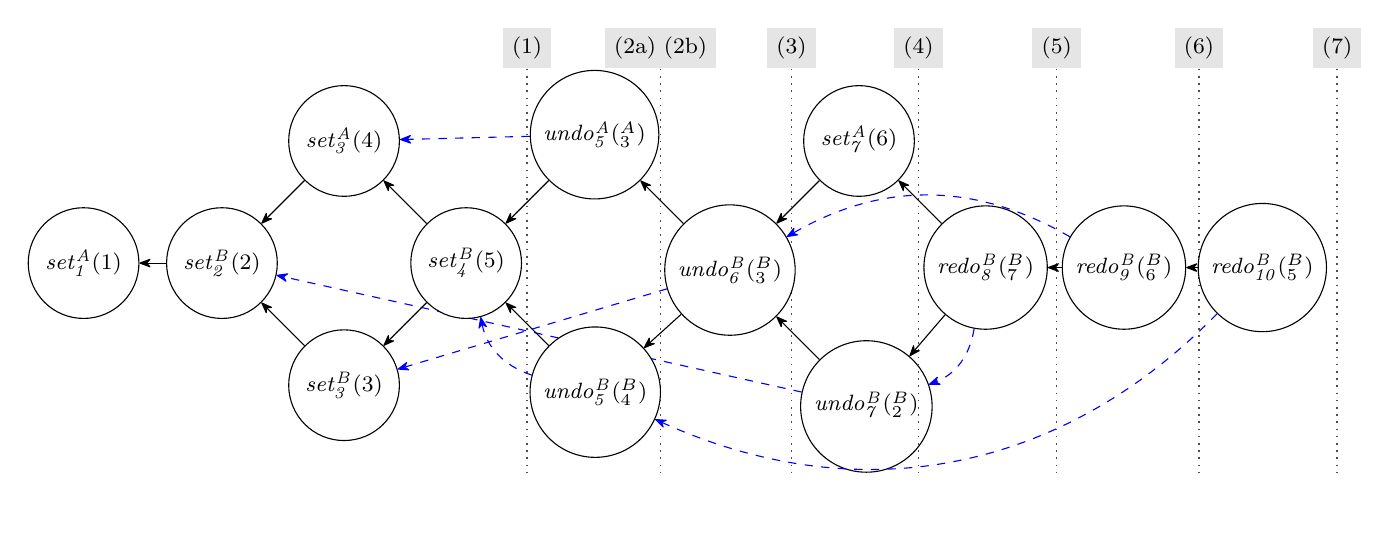
\begin{tikzpicture}[node distance=50pt]
  \def\dist{22pt}

  % nodes and edges
  \node[op] (a1) at (0, 0) {\setop{1}{A}{1}};
  \node[op,right of=a1] (b2) {\setop{2}{B}{2}} edge [pred] (a1);

  \node[op,above right=\dist of b2] (a3) {\setop{3}{A}{4}} edge [pred] (b2);
  \node[op,below right=\dist of b2] (b3) {\setop{3}{B}{3}} edge [pred] (b2);

  \node[op,below right=\dist of a3] (b4) {\setop{4}{B}{5}} edge [pred] (b3) edge [pred] (a3);

  \node[op,above right=\dist of b4] (a5) {\undop{5}{A}{3}{A}} edge [pred] (b4) edge [anchorref] (a3);
  \node[op,below right=\dist of b4] (b5) {\undop{5}{B}{4}{B}} edge [pred] (b4) edge [anchorref,bend left] (b4);

  \node[op,below right=\dist of a5] (b6) {\undop{6}{B}{3}{B}} edge [pred] (b5) edge [pred] (a5) edge [anchorref] (b3);

  \node[op,above right=\dist of b6] (a7) {\setop{7}{A}{6}} edge [pred] (b6);
  \begin{scope}[on background layer]
  \node[op,below right=\dist of b6] (b7) {\undop{7}{B}{2}{B}} edge [pred] (b6) edge [anchorref] (b2);
  \end{scope}

  \node[op,below right=\dist of a7] (b8) {\redop{8}{B}{7}{B}} edge [pred] (b7) edge [pred] (a7) edge [anchorref,bend left] (b7);

  \node[op,right of=b8] (b9) {\redop{9}{B}{6}{B}} edge [pred] (b8) edge [anchorref,bend right=30] (b6);

  \node[op,right of=b9] (b10) {\redop{10}{B}{5}{B}} edge [pred] (b9) edge [anchorref,bend left=35] (b5);

  % step marker and step lines
  \begin{scope}[on background layer]
  \def\divlen{155pt}

  \node[stepmarker,above=50pt of b4,xshift=+22.0pt] (1) {(1)} edge [stepline] ($ (1.center)-(0,\divlen) $);

  \node[stepmarker,right=19.0pt of 1] (2a2b) {(2a) (2b)} edge [stepline] ($ (2a2b.center)-(0,\divlen) $);

  \node[stepmarker,right=18.0pt of 2a2b] (3) {(3)} edge [stepline] ($ (3.center)-(0,\divlen) $);

  \node[stepmarker,right=28.0pt of 3] (4) {(4)} edge [stepline] ($ (4.center)-(0,\divlen) $);

  \node[stepmarker,right=32.0pt of 4] (5) {(5)} edge [stepline] ($ (5.center)-(0,\divlen) $);

  \node[stepmarker,right=33.5pt of 5] (6) {(6)} edge [stepline] ($ (6.center)-(0,\divlen) $);

  \node[stepmarker,right=32.0pt of 6] (7) {(7)} edge [stepline] ($ (7.center)-(0,\divlen) $);

  \end{scope}
\end{tikzpicture}
\caption{
An operation history which is replicated between two actors A and B that includes
undo and redo operations. For clarity, undo and redo operations are not labeled
as \restopkind{}s. Their respective anchor operations are indicated by the
dashed blue arrows and denoted in parenthesis.
The dotted lines indicate time steps during which we show the nodes' states in
\cref{tab:node-states}.
}\label{fig:op-hist-undo-redo}
\end{figure*}

\newcommand{\ra}[1]{\renewcommand{\arraystretch}{#1}}

\begin{table*}[h!]
  \centering
  \small
  \ra{1.3}
  \begin{tabular}{@{}llllllllll@{}}
    \toprule
      Time Step 
        & (1)
        & (2a)
        & (2b)
        & (3)
        & (4)
        & (5)
        & (6)
        & (7)
        \\
    \midrule
      $\mathit{undo Stack}^A$
        & \stack{\setop[\setabbr]{1}{A}{1},\setop[\setabbr]{3}{A}{4}}
        & \stack{\setop[\setabbr]{1}{A}{1}}
        & (2a)
        & (2a)
        & \stack{\setop[\setabbr]{1}{A}{1},\setop[\setabbr]{7}{A}{6}}
        & (4)
        & (4)
        & (4)
        \\
      $\mathit{redo Stack}^A$
        & \stack{}
        & \stack{\restop[\restabbr]{5}{A}{3}{A}}
        & (2a)
        & (2a)
        & \stack{}
        & (4)
        & (4)
        & (4)
        \\
      $\mathit{register}^A$
        & \stack{5}
        & \stack{2}
        & \stack{3,4,2}
        & \stack{2}
        & \stack{1,6}
        & \stack{2}
        & \stack{3,4,2}
        & \stack{5}
        \\
    \midrule
      $\mathit{undo Stack}^B$
        & \stack{\setop[\setabbr]{2}{B}{2},\setop[\setabbr]{3}{B}{3},\setop[\setabbr]{4}{B}{5}}
        & \stack{\setop[\setabbr]{2}{B}{2},\setop[\setabbr]{3}{B}{3}}
        & (2a)
        & \stack{\setop[\setabbr]{2}{B}{2}}
        & \stack{}
        & (3)
        & (2a)
        & (1)
        \\
      $\mathit{redo Stack}^B$
        & \stack{} 
        & \stack{\restop[\restabbr]{5}{B}{4}{B}}
        & (2a)
        & \stack{\restop[\restabbr]{5}{B}{4}{B},\restop[\restabbr]{6}{B}{3}{B}}
        & \stack{\restop[\restabbr]{5}{B}{4}{B},\restop[\restabbr]{6}{B}{3}{B},\restop[\restabbr]{7}{B}{2}{B}}
        & (3)
        & (2a)
        & (1)
        \\
      $\mathit{register}^B$   
        & \stack{5}
        & \stack{3,4}
        & \stack{3,4,2}
        & \stack{2}
        & \stack{1,6}
        & \stack{2}
        & \stack{3,4,2}
        & \stack{5}
        \\
    \bottomrule
  \end{tabular}
\caption{
The internal states of the nodes' undo and redo stacks and the values of the register
at the time steps from \cref{fig:op-hist-undo-redo}.
A set operation is abbreviated by $\mathit{\setabbr}$ and a restore operation
by $\mathit{\restabbr}$
with its anchor operation denoted within parenthesis.
In case a cell contains a reference to another time step, the value is exactly
the same as in that respective step.
The difference between (2a) and (2b) is that in (2a) both replicas have not yet
synced whereas in (2b) they have exchanged their operations.
At all other time steps the operations are assumed to be synced.
}\label{tab:node-states}
\end{table*}

\Cref{fig:op-hist-undo-redo} shows an operation history that is replicated
between two actors $A$ and $B$ that contains undo and redo operations.
\Cref{tab:node-states} shows the internal node states during the time steps
from \cref{fig:op-hist-undo-redo}.
It demonstrates the stack maintenance introduced in \cref{sec:overview} and
shows the register's values produced by
\cref{alg:core-alg,alg:gen-values,alg:comparison-fn} which are applied on top
of the respective operation histories at the time steps.
Steps (2a) and (2b) point out how two concurrent undo operations are resolved.
\undop{5}{A}{3}{A} produces the value $2$ with an \opidtrace{} of
\stack{\opid{5}{A},\opid{2}{B}}.
\undop{5}{B}{4}{B} produces the values $3$ with an \opidtrace{} of
\stack{\opid{5}{B},\opid{3}{B}}
and $4$ with an \opidtrace{} of
\stack{\opid{5}{B},\opid{3}{A}}.
Sorting by these \opidtrace{}s yields the register's values \stack{3,4,2}
after syncing in (2b).

The concurrent \undop{7}{B}{2}{B} and \setop{7}{A}{6} operations at (4) highlight
the requirement of the \opidtrace{}.
The \undop{7}{B}{2}{B} operation produces the value $1$ with an \opidtrace{} of
\stack{\opid{7}{B},\opid{1}{A}}.
The \setop{7}{A}{6} operation immediately yields the value $6$ with an
\opidtrace{} of \stack{\opid{7}{A}}.
If there was no \opidtrace{} and instead the \glspl*{opid} of the terminal
operations were used, the values produced by the undo operation would
always lose against the concurrent set operation because the \glspl*{opid} of the
terminal operations are always smaller than the \gls*{opid} of the concurrent
set operation due the traversal of the predecessor relation.
To fix this unfairness, the \opidtrace{} is employed to sort values produced by
\emph{different heads} by their head's \glspl*{opid} and
values produced by the \emph{same head}
by their first deviation in the \opidtrace{}.

Finally, at (4) $A$ is giving up its ability to redo because its terminal
operation \setop{7}{A}{6} clears the redo stack, rendering $A$ unable to redo its
previously undone \setop{3}{A}{4} operation.

\section{Optimization}\label{sec:opt}

%% TODO: put this in the evaluation section?

We can make use of two observations to optimize the algorithm:
First, the predecessors of an operation remain constant after their generation.
Incoming concurrent operations may have existing operations as their predecessors
but they never update the predecessors of existing operations.
Second, a \restopkind{}'s anchor is also fixed at generation time.
As explained in \cref{sec:evaluation}, there are degenerate cases in which after
following the anchor and resolving its predecessors, one predecessor is another
\restopkind{} and the same pattern repeats for a few iterations,
leading to a non-constant runtime.
Yet, due to the two key observations above, we are resolving the exact same values
for a \restopkind{} which we have already resolved at the time it was the head of
the operation history.
Hence, we can harness caching to improve the runtime at the expense of an
increased memory overhead.

For each \restopkind{} we cache the values produced by it in sorted order.
As soon we have stored the sorted order, we can even drop the \opidtrace{} and rely
on a \emph{stable} sort algorithm to include the sorted values of a \restopkind{}
at the right position with just the \opidtrace{} up to the \restopkind{}'s \gls*{opid}.
This works because if a \restopkind{} produces multiple values, the part of the \opidtrace{}
going beyond the \restopkind{} is responsible for sorting the values it produces.
Storing the values in sorted order makes that part of the \opidtrace{} redundant.
Only the first part of the \opidtrace{} up to the \restopkind{} is important for figuring
out the relation of the cached values with other values contributed by other operations.
However, this requires the sorting algorithm to be stable.

\section{Evaluation}\label{sec:evaluation}

% Explain the high-level research questions
% Experimental testbed, benchmarks, methodology
% Evaluate the research questions/hypotheses

\begin{figure*}[ht!]
\centering
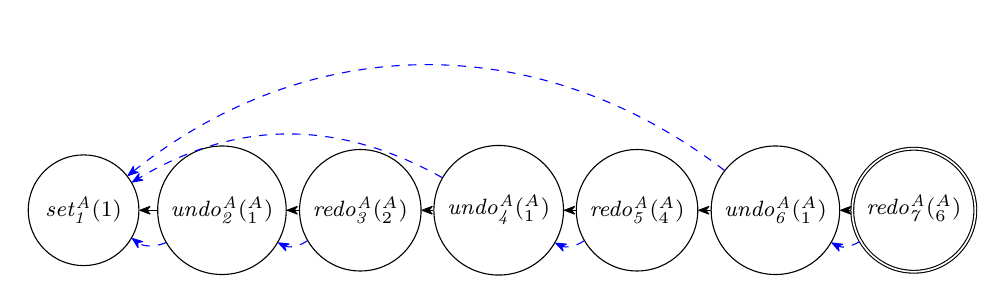
\begin{tikzpicture}[node distance=50pt]

  % nodes and edges
  \node[op] (a1) at (0, 0) {\setop{1}{A}{1}};
  \node[op,right of=a1] (a2) {\undop{2}{A}{1}{A}} edge [pred] (a1) edge [anchorref,bend left] (a1);
  \node[op,right of=a2] (a3) {\redop{3}{A}{2}{A}} edge [pred] (a2) edge [anchorref,bend left] (a2);
  \node[op,right of=a3] (a4) {\undop{4}{A}{1}{A}} edge [pred] (a3) edge [anchorref,bend right] (a1);
  \node[op,right of=a4] (a5) {\redop{5}{A}{4}{A}} edge [pred] (a4) edge [anchorref,bend left] (a4);
  \node[op,right of=a5] (a6) {\undop{6}{A}{1}{A}} edge [pred] (a5) edge [anchorref,bend right=38] (a1);
  \node[head,right of=a6] (a7) {\redop{7}{A}{6}{A}} edge [pred] (a6) edge [anchorref,bend left] (a6);

\end{tikzpicture}
\caption{
  A sequence of alternating undo-redo operations
  of length $3$ (counting one undo-redo-pair as one).
  In this case, the algorithm's run time is not constant but linear
  in the length of the sequence.
}\label{fig:degenerate-op-sequence}
\end{figure*}

To evaluate the correctness of our algorithm, we demonstrate that it converges,
and we check the behavior of our reference implementation with a suite of unit tests.
To evaluate its performance, we analyze its runtime complexity for relevant
undo and redo scenarios and provide benchmarking results.
Finally, we discuss its integration with Automerge.

\textbf{Correctness}.
We demonstrate that any two replicas that have received the same set of
operations converge to the same state.
The same set of operations produce the same operation history on both
replicas over which the algorithms from \cref{sec:implementation} are applied.
Since the algorithms are deterministic and do not depend on the order in which
operations were received, they produce the same value(s) on both
replicas, given that they terminate.
\Cref{alg:gen-values}'s termination is trivial since it sorts and then
maps a finite set of operations.
The termination of the comparison function from \cref{alg:comparison-fn} is
guaranteed by the fact that \opidtrace{}s are finite
(due to the operation history being finite).
\Cref{alg:core-alg}'s termination is a bit more involved.
If all heads are terminal operations, termination is trivial as in the 
while loop, the length of the \textit{todo} list decreases by one in every iteration
and no element is inserted.
When dealing with \restopkind{}s, in every iteration of the while loop
the length of the \textit{todo} list also decreases by one but it also 
increases by the number of predecessors of the anchor operation.
Yet, due to the operation history being finite, cycle-free and \autoref{alg:core-alg}
going only backwards in time but never forwards
(by following the predecessor relation in case of \restopkind{}s),
termination is guaranteed.
Therefore, the algorithm converges to the same state on both replicas.

The reference implementation is written in Typescript and consists of around 350
lines of code (excluding comments and blank lines),
implementing an \gls*{mvr} with undo and redo functionality as described
in \cref{sec:background,sec:overview,sec:implementation}.
The implementation is tested against a set of unit tests that covers important
scenarios, both in single-user and multi-user cases.
In total there are 30 unit tests,
comprising of around 640 lines of test code (also excluding comments and blank lines).

\textbf{Performance}.
\autoref{alg:gen-values}'s runtime is entirely driven by the
complexity of sorting the terminal operations and \cref{alg:comparison-fn}'s
runtime is linear in the length of the shorter \opidtrace{}.
To assess \autoref{alg:core-alg}'s runtime,
we look at the runtime of resolving the different operation kinds,
\setopkind{} and \restopkind{}.
To ease the analysis, we ignore any complexity arising from dealing with
data structures like maps and lists but focus on the iterations
of the while loop in lines 4-12.
In case of a \setopkind{}, the runtime is constant as the while loop
does not add an element to the \textit{todo} list but just removes the
\setopkind{} from the list.

For \restopkind{}s, we push all $k$ predecessors of the referenced anchor operation
to the \textit{todo} list and therefore have to process $k$ more operations.
Some of these $k$ operations may be \setopkind{}s which end the search but
some may be \restopkind{}s themselves. 
Then, the process repeats until a terminal operation is found or
roots are reached that cannot add any predecessors to the \textit{todo} list.
The amount of predecessors depends on the degree of concurrency in the system.
We restrict the analysis to linear operation histories and therefore assume
that there is just one predecessor of a \restopkind{}.
Nevertheless, the following arguments can still be applied for each branch
introduced by a predecessor of a \restopkind{}, albeit with a shorter length.

In most practical editing scenarios,
the resolution of a \restopkind{} head to a value happens in constant time.
For example, if a user performs $n$ undo operations (to see prior document states)
followed by $m \leq n$ redo operations (to return to one of the document states),
the resolution of each undo and redo operation happens in constant time,
provided that the anchor operations' predecessor of the $n$ undo operations
are all terminal operations.
In that case each undo operation resolves to a terminal operation in two iterations
(one for its \restopkind{} and its anchor's predecessor (a terminal operation))
and each redo operation resolves
to a terminal operation in three iterations
(one for its \restopkind{}, its anchor's
predecessor (an undo operation) and that undo operation's predecessor of its anchor
(a terminal operation)).

However, there are scenarios where the resolution of a \restopkind{} head
to a value is not constant but linear in the length
of the (per assumption linear) operation history.
\Cref{fig:degenerate-op-sequence} shows such a scenario where a single actor
produces an operation history of alternating undo-redo operations.
For resolving the head of a sequence of alternating undo-redo operations
of length $n$ (counting one undo-redo-pair as one),
the algorithm has to iterate $n$ times to find the terminal operation.
Yet, only the resolution of a redo operation suffers from this whereas
the resolution of an undo operation still happens in constant time.
The same effect can be created by alternating set and undo operations.
Yet in practice, this is not a real concern as we expect the lengths of such
degenerate sequences to be limited as undo and redo is a human-facing feature.
More importantly, we think that neither alternating undo and redo
nor set and undo operations is a common use case.

Benchmarks of our reference implementation support these findings.
\Cref{fig:runtime-cons-undo-redo} and \cref{fig:runtime-undo-redo-alt} measure
the runtime in two different scenarios for undo and redo.
Each data point shows the mean runtime over 1024 runs.
The benchmarking was conducted on a 2019 MacBook Pro with a 
2.6 GHz 6-Core Intel Core i7 processor and Node version 18.17.1.

\begin{figure}
  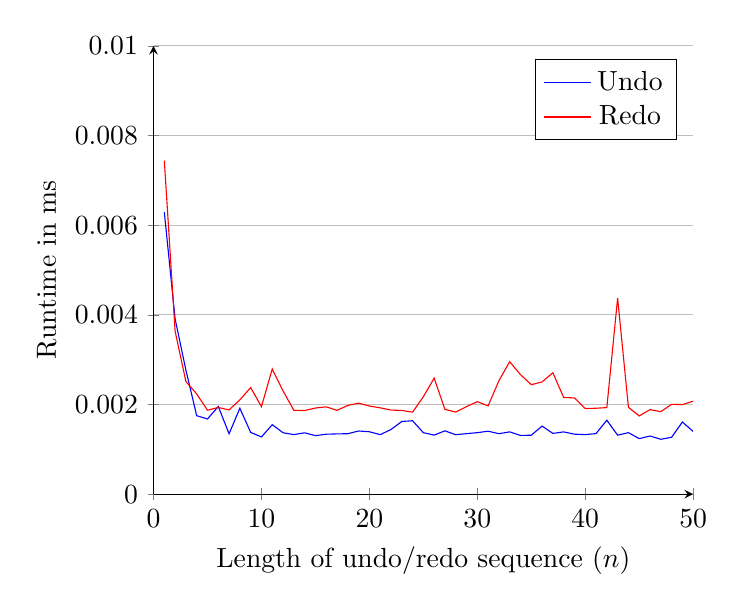
\begin{tikzpicture}
  \begin{axis}[
    xlabel={Length of undo/redo sequence ($n$)},
    ylabel={Runtime in ms},
    xmin=0,
    axis x line=bottom,
    axis y line=left,
    ymin=0,
    ymax=0.01,
    legend pos=north east,
    ymajorgrids=true,
    yticklabel style={
      /pgf/number format/fixed,
      /pgf/number format/precision=5
    },
    scaled y ticks=false 
  ]

  % undo data
  \addplot[
    color=blue,
  ] coordinates {
(1, 0.006290340563282371)
(2, 0.003907741687726229)
(3, 0.002766803983831778)
(4, 0.0017496687069069594)
(5, 0.0016760083672124892)
(6, 0.001955396990524605)
(7, 0.001345782628050074)
(8, 0.0019154881010763347)
(9, 0.0013770495424978435)
(10, 0.001276014547329396)
(11, 0.0015485882759094238)
(12, 0.0013692353677470237)
(13, 0.0013271856296341866)
(14, 0.0013679209514521062)
(15, 0.001304528908804059)
(16, 0.0013366359926294535)
(17, 0.0013435808941721916)
(18, 0.00134780234657228)
(19, 0.0014081033586990088)
(20, 0.0013913525617681444)
(21, 0.0013268127804622054)
(22, 0.001440957625163719)
(23, 0.0016200695536099374)
(24, 0.0016375818522647023)
(25, 0.0013710299390368164)
(26, 0.0013164350239094347)
(27, 0.0014119130210019648)
(28, 0.0013253243814688176)
(29, 0.0013492428988683969)
(30, 0.0013712448126170784)
(31, 0.0014037845248822123)
(32, 0.0013481056957971305)
(33, 0.0013890777481719851)
(34, 0.0013086109538562596)
(35, 0.001314542896579951)
(36, 0.0015176087035797536)
(37, 0.0013542969536501914)
(38, 0.0013883131032343954)
(39, 0.0013373843976296484)
(40, 0.0013278163387440145)
(41, 0.0013506945979315788)
(42, 0.0016484785883221775)
(43, 0.0013150325394235551)
(44, 0.0013713290682062507)
(45, 0.0012379433319438249)
(46, 0.0012963268964085728)
(47, 0.0012237174669280648)
(48, 0.0012681810767389834)
(49, 0.001609297381946817)
(50, 0.0013969987630844116)
    };

  % redo data
  \addplot[
    color=red,
  ] coordinates {
(1, 0.007437939144438133)
(2, 0.003633987420471385)
(3, 0.002511455590138212)
(4, 0.0022350119543261826)
(5, 0.0018720132065936923)
(6, 0.0019328816561028361)
(7, 0.00187860953155905)
(8, 0.002103224309394136)
(9, 0.0023768509563524276)
(10, 0.001951182057382539)
(11, 0.0027914689562749118)
(12, 0.002302225591847673)
(13, 0.0018702853412833065)
(14, 0.001864643389126286)
(15, 0.0019206689321435988)
(16, 0.0019472866551950574)
(17, 0.0018687470292206854)
(18, 0.0019792676030192524)
(19, 0.002029231225606054)
(20, 0.001964766182936728)
(21, 0.0019252107886131853)
(22, 0.0018749097071122378)
(23, 0.001866210310254246)
(24, 0.0018289572326466441)
(25, 0.0021713866444770247)
(26, 0.002587106981081888)
(27, 0.0018908421625383198)
(28, 0.0018309024162590504)
(29, 0.0019520004279911518)
(30, 0.002062761748675257)
(31, 0.001968364085769281)
(32, 0.002528973447624594)
(33, 0.002954049239633605)
(34, 0.0026645801845006645)
(35, 0.002441259188344702)
(36, 0.002502664952771738)
(37, 0.002708020620048046)
(38, 0.002156659436877817)
(39, 0.0021457494294736534)
(40, 0.0019089243141934276)
(41, 0.0019161189266014844)
(42, 0.0019302570726722479)
(43, 0.004374536831164733)
(44, 0.0019373227842152119)
(45, 0.0017444676195736974)
(46, 0.0018851725617423654)
(47, 0.001839210162870586)
(48, 0.0020025315461680293)
(49, 0.0019971978035755455)
(50, 0.002073564799502492)
  };

  \legend{Undo, Redo}

  \end{axis}
  \end{tikzpicture}
\caption{
  Runtime of the last undo (redo) operation in a sequence
  of $n$ consecutive set operations followed by $n$ undo operations
  ($n$ consecutive set operations followed by $n$ undo operations
   followed by $n$ redo operations).
}\label{fig:runtime-cons-undo-redo}
\end{figure}

\Cref{fig:runtime-cons-undo-redo} covers the undo-redo-neutrality principle
from \cref{sec:semantics}.
For undo operations, the mean runtime of generating and applying an undo
operation is shown with $n-1$ preceding undo operations
which are in turn preceded by $n$ set operations, for $n \in \{1,2,\ldots,50\}$.
For redo operations, the undo sequence is extended by $n$ redo operations.
Similarly, it shows the mean runtime of generating and applying the last redo
operation.
Both undo and redo runtimes are mostly constant and therefore independent of the
length of the sequence.
We suspect that the initial spike of both undo and redo is due to Node's
just-in-time compilation not yet having optimized the code.
The outlier for redo operations at $n = 43$ may be explained by a garbage collection pause.
Redo operations take slightly longer than undo operations for two reasons.
First, a redo operation resolves its anchor operation to a terminal operation
and puts it onto the undo stack for possibly undoing it later again, whereas
an undo operation just puts its \restopkind{} onto the redo stack.
Second, resolving to a terminal operation takes three iterations for a redo operation
as opposed to just two iterations for an undo operation.

\begin{figure}
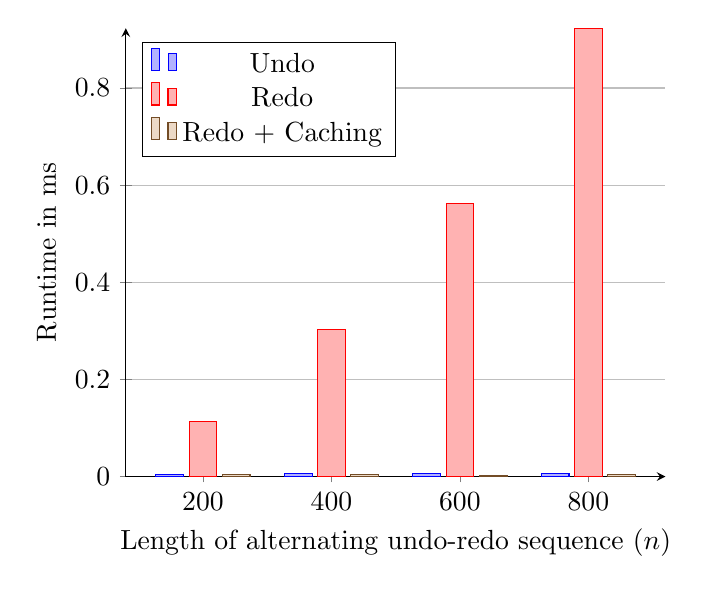
\begin{tikzpicture}
\begin{axis}[
  ybar,
  ylabel={Runtime in ms},
  axis y line=left,
  ymin = 0,
  xlabel={Length of alternating undo-redo sequence ($n$)},
  axis x line=bottom,
  symbolic x coords={200, 400, 600, 800},
  ymajorgrids=true,
  yminorgrids=true,
  enlarge x limits = 0.2,
  legend pos = north west,
] 

% undo
\addplot+ coordinates {
(200, 0.00504857866326347)
(400, 0.005509669485036284)
(600, 0.006512108666356653)
(800, 0.007120864116586745)
};

% redo without cache opt
\addplot+ coordinates {
(200, 0.11390662190387957)
(400, 0.3034253417572472)
(600, 0.5630059454997536)
(800, 0.9230491668859031)
}; 

% redo with cache opt
\addplot+ coordinates {
(200, 0.0034364885359536856)
(400, 0.00369966629659757)
(600, 0.0026536431978456676)
(800, 0.0034199498768430203)
};

\legend{Undo, Redo, Redo + Caching};
\end{axis} 
\end{tikzpicture} 
\caption{
  Runtime of the last undo/redo operation
  in a sequence of alternating undo-redo operations of length $n$
  (counting one undo-redo-pair as one; see \cref{fig:degenerate-op-sequence}).
}\label{fig:runtime-undo-redo-alt}
\end{figure}

\Cref{fig:runtime-undo-redo-alt} illustrates the mean runtime of the last
undo or redo operation of a sequence of alternating undo-redo operations
of length $n$ for $n \in \{200, 400, 600, 800\}$.
This scenario resembles \cref{fig:degenerate-op-sequence}, but with longer sequences,
and measures the time to generate and apply the head of the sequence.
As previously discussed, the runtime of undo operations is constant in this
scenario and not affected by the length of the sequence.
The runtime of applying redo operations grows linearly with the length of the sequence.
With $n = 800$, applying the redo head takes 0.9 milliseconds.
We believe that this does not impact the user experience negatively,
since the user will not notice a delay of less than a millisecond and the use
of a compiled language like Rust may further reduce the runtime.
Finally, we consider an alternating undo-redo sequence of length 800 irrelevant
in practice.

\textbf{Integration with Automerge}.
Since Automerge stores a monotonically growing set of operations,
efficient compression of the serialized operation set is an important property.
Our proposed solution models both undo and redo with a single
operation kind whose extra payload consists only of a single \gls*{opid}.
Moreover, the \restopkind{} may also be useful to support global undo
behavior in addition to local undo in the future.
Since every undo and redo creates a new \restopkind{} that is added
to the set,
the undo and redo stacks are implicitly stored within the operation set and
can be reconstructed upon loading the document to support undo and redo
across sessions without any additional persistency overhead.

Moreover, if an application developer decides not to use undo and redo functionality,
the value resolution algorithm will be the same as without undo and redo functionality,
thereby not incurring any overhead and making users of the library only
pay for what they use.
In terms of space complexity, the additional overhead is the introduced state
of the undo and redo stacks which can be disabled if not needed and are otherwise
just a fraction of the total number of operations of the register and can be
bounded if arbitrary undo depth support is not required.

Finally, we remark a possibility to prune the history under a special circumstance.
Imagine a user undoing a few times and then redoing the same amount of times
just to see the document in the past and then return to the original state.
We call such a sequence of undo and redo operations effect-free.
Given that all participating actors have seen the same operations and made no
changes to the register within the effect-free sequence,
the sequence can be pruned (garbage collected) from the history.
However, before doing so causal stability~\cite{baquero2017pure}
must be reached, that is, all
actors must have sent an operation whose predecessor set contains the
highest \gls*{opid} of the effect-free sequence.

\section{Related Work}\label{sec:related-work}

%% TODO: y.js code review

The terms local and global undo were introduced by the \acrlong{ot}
literature in the context of collaborative text
editing~\cite{sun2000undo,ressel1999reducing, abowd1992giving},
but this distinction is less established in the context of \glspl{crdt}.

A common approach to undo and redo in the \gls{crdt} literature is
to attach a counter
(sometimes called \emph{degree}~\cite{Weiss2010LogootUndo} or
\emph{undo length}~\cite{Brattli2021undo,Yu2019undo}) to each operation.
Some approaches~\cite{Weiss2010LogootUndo,Martin2010xml} initialize the
counter to $1$ and decrement it on each undo and increment it on each redo.
If the counter is positive, the operation is visible,
otherwise it is invisible.
Other approaches~\cite{Brattli2021undo,Yu2019undo} initialize the counter
to $0$ and increment it on each undo and redo.
If it is even, the operation is visible, otherwise it is not.
When merging conflicting counters of an operation, the maximum is used.
Yet, counter-based approaches handle undo only for a single operation
and do not allow skipping over remote operations, which is required
for local undo behavior as we pointed out in \cref{sec:semantics}.
To illustrate this we consider \cref{fig:anti-counter}.
It resembles the single-register scenario in \cref{fig:intro-example} but
instead of $A$ redoing in the last step, $B$ issues an undo.
\Cref{fig:anti-counter} shows the correct outcomes according to local undo
behavior.
Applying counter-based approaches to this scenario poses some challenges.
$A$'s undo would render both $A$'s and $B$'s \setopkind{} invisible to
achieve the correct black coloring of the rectangle (step (4)).
$B$'s subsequent undo requires to turn $A$'s \setopkind{} visible again to
obtain the correct red coloring (step (5)).
To achieve this, $B$'s \emph{undo} must cause the effect of a \emph{redo}
of $A$'s \setopkind{}.
Since this simple example is already difficult (and not even considering
concurrency), we believe that counter-based approaches are not suitable
for implementing local undo.

%% TODO: add further example with concurrency

\begin{figure}
\centering
\begin{tikzpicture}[node distance=0.23cm]
  \coordinate (c1) at (0,0);

  \tikzset{
    canvas/.style={
      rectangle,
      draw,
      anchor = west,
      inner sep = 4pt,
    },
    rect/.style={
      rectangle,
      minimum width = 1.2cm, 
      minimum height = 0.5cm,
      inner sep = 0.1cm,
      text = white,
      fill = #1,
    },
    optrans/.style={
      <-,bend right=90,>={Stealth[round]},
      swap,
      black!70,
    },
    casediv/.style={
      black!70,
    },
  }

  \def\black{black}
  \def\green{green!60!black}
  \def\red{red}
  \def\upperoffset{8pt}

  % divider lines and ops

  \coordinate (d1s) at ($(a1.north)!0.5!(a2.north)+(0,+\upperoffset)$);
  \coordinate (da5) at ($(e1.south)!0.5!(e2.south)+(0,0)$);

  \coordinate (d2s) at ($(a2.north)!0.5!(a3.north)+(0,+\upperoffset)$);
  \coordinate (db5) at ($(e2.south)!0.5!(e3.south)+(0,0)$);

  \coordinate (d3s) at ($(a3.north)!0.5!(a4.north)+(0,+\upperoffset)$);
  \coordinate (dc5) at ($(e3.south)!0.5!(e4.south)+(0,0)$);

  \coordinate (d4s) at ($(a4.north)!0.5!(a5.north)+(0,+\upperoffset)$);
  \coordinate (dd4) at ($(e4.south)!0.5!(e5.south)+(0,0)$);

  \draw[stepline] (d1s) -- (da5);
  \draw[stepline] (d2s) -- (db5);
  \draw[stepline] (d3s) -- (dc5);
  \draw[stepline] (d4s) -- (dd4);

  \draw (a2.north)+(-0.2cm,+\upperoffset) edge ["A set",optrans] ($(a1.north)+(0,+\upperoffset)$);
  \draw (a3.north)+(-0.2cm,+\upperoffset) edge ["B set",optrans] ($(a2.north)+(0,+\upperoffset)$);
  \draw (a4.north)+(-0.2cm,+\upperoffset) edge ["A undo",optrans] ($(a3.north)+(0,+\upperoffset)$);
  \draw (a5.north)+(-0.2cm,+\upperoffset) edge ["A redo",optrans] ($(a4.north)+(0,+\upperoffset)$);

  %%%%
  
  \node[
    canvas,
    label={[]above:(1)},
  ] (2a) at (c1) {
    \begin{tikzpicture}[node distance=3pt]
      \node[
          rect=\black,
        ] (r1) at (0,0) {\vphantom{bg}black};
    \end{tikzpicture}
  };

  \node[
    canvas,
    label={[]above:(2)},
    right = of 2a,
  ] (2b) {
    \begin{tikzpicture}[node distance=3pt]
      \node[
          rect=\red,
        ] (r1) at (0,0) {\vphantom{bg}red};
    \end{tikzpicture}
  } edge (2a);

  \node[
    canvas,
    label={[]above:(3)},
    right = of 2b,
  ] (2c) {
    \begin{tikzpicture}[node distance=3pt]
      \node[
          rect=\green,
        ] (r1) at (0,0) {\vphantom{bg}green};
    \end{tikzpicture}
  } edge (2b);

  %%%

  \node[
    canvas,
    label={[]above:(4)},
    right = of 2c,
  ] (2d1) {
    \begin{tikzpicture}[node distance=3pt]
      \node[
          rect=\black,
        ] (r1) at (0,0) {\vphantom{bg}black};
    \end{tikzpicture}
  } edge (2c);

  \node[
    canvas,
    label={[]above:(5)},
    right = of 2d1,
  ] (2d1e2) {
    \begin{tikzpicture}[node distance=3pt]
      \node[
          rect=\red,
        ] (r1) at (0,0) {\vphantom{bg}red};
    \end{tikzpicture}
  } edge (2d1);

\end{tikzpicture}
\caption{
  A simple but challenging scenario for counter-based approaches if local undo
  behavior is desired.
}\label{fig:anti-counter}
\end{figure}

Yu et al.~\cite{Yu2015undo} deal with selective undo in the context of strings.
Selective undo is a form of undo which allows a user to undo any operation,
regardless of \emph{where and when} it was generated.
In contrast, global undo allows undoing a remote operation as well,
but it only allows undoing in reverse chronological order.
A later work of Yu et al.~\cite{Yu2019undo} describes a generic undo mechanism,
but it only applies to state-based \glspl*{crdt}, is assuming global undo
behavior, and focusses on concurrent undo and redo of a single operation.
It does not address the issue of how to order operations on the undo
stack with global undo.

Finally,~\cite{Dolan2020undoable} is a rather theoretical work that
points out limitations of undo for set and counter \glspl*{crdt}.
Martin et al.~\cite{Martin2010xml} discuss undo in the context of XML-like documents.
To the best of our knowledge, Brattli et al.~\cite{Brattli2021undo} is the
only work that also discusses undo and redo in the context of replicated registers,
but they assume global undo behavior.

\section{Conclusion}\label{sec:conclusion}

We tested the semantics of undo and redo of existing collaboration software,
and found that almost all use local undo.
We then presented a novel algorithm for local undo on an \gls*{mvr}
by traversing operation histories represented as directed acyclic graphs.
The Automerge \gls{crdt} implementation already stores such an operation graph
to allow past states of a document to be inspected;
therefore our algorithm does not incur any additional overhead in this context.
The implementation of our algorithm is currently a standalone prototype
written in Typescript, but we plan to integrate it into Automerge in the future.
We believe that our algorithm can also be generalized from a single \gls{mvr}
to more complex \glspl{crdt}, for example by treating every key in a map and
every element in a list as a \gls{mvr}, and by using (respectively) one shared
undo and redo stack for all \glspl{mvr} in the entire data structure.

%%
%% Print the bibliography
\printbibliography

%%
%% If your work has an appendix, this is the place to put it.
\appendix

\section{Challenges with Global Undo}\label{adx:global-undo-challenges}

Although we argued against the behavior of global undo, we put forward
some considerations if using it in an eventually consistent setting that
allows for operations to arrive in causal (or even arbitrary) order.

\subsection{Undo Order}

In general, an undo mechanism requires some order to determine which
operation(s) to undo next. 
While this does not have to be a total order and
one could come up with a scheme how to undo a partial order,
the eventual consistent setting poses a technical limit:
Suppose there is a sequence of undo operations and the first undone operation
has timestamp $t_f$ and the last undone operation $t_l$.
Then, an operation is delivered out-of-order with
timestamp $t_m$ such that $t_l < t_m < t_f$ according to the (partial) order.
This means that \emph{if} the out-of-order operation had been delivered earlier it
had also been undone by the undo sequence.
We call such operations \emph{out-of-order delivered and behind the undo cursor}.
This leaves the question of how to treat these operations.
A potential solution is to turn the undo stack into a priority queue and
then undo the operation at the time of arrival at the undoing actor but
that may cause hard to understand jumps in time for users.
Another option is to ignore these operations but that poses the issue of
how to deal with them upon subsequent redos.
We are not convinced of any good solution here and think of this as another,
rather technical reason to avoid global undo behavior in eventually consistent
settings.

Nevertheless, we briefly sketch a scheme how to undo a partial order.
The idea is to use multiple cursors that undo in parallel whenever the
partial order cannot compare operations (due to concurrency).
After a merge operation is undone, assume there are multiple branches
that are candidates to undo next.
For each branch a cursor pointing to the next operation that is due for undo
is created and it initially points to the respective tip of the branch.
Upon undo, the \gls{mvr} is populated with all values contributed by the
operations referenced by the cursors, and the cursors are advanced
to point to their predecessors.
Different strategies may be employed to coordinate the cursors in case
any cursor hits a common ancestor or another merge operation.

If the increased complexity from the cursor handling is undesired,
the total order imposed by the operation ids could also be used.
However, the out of order delivery issue remains for both total and
partial orders.
In contrast, local undo restricts the undoable operations to the subset of
the actor's own operations which are always delivered in order at each actor,
and thereby does not suffer from this problem.

\subsection{Metadata Overhead}

Local undo partitions the set of operations into disjoint sets,
one set for each actor.
Since an actor can only undo her own operations,
it cannot happen that concurrently the same operation is undone multiple times,
or that the same operation is both undone and redone by different actors.
While it certainly is possible to design some data structure to account for this,
it increases the complexity and overhead of the algorithm.

\end{document}
\endinput
